\subsubsection{Choix de l'algorithme}

Pour le calcul du plus court chemin nous avons fait le choix d'appliquer l'algorithme de Dijkstra. C'est un algorithme simple, efficace et que nous avons vu cours de Recherche Operationnelle. Pour l'implémentation nous avons créé un package Djikstra comportant les classes suivantes:
\begin{itemize}
	\item Vertex: cette classe correspond au noeuds du graphe utilisé pour l'algorithme;
	\item Edge: cette classe correspond au arc entre 2 noeuds adjacents;
	\item Djikstra: cette classe permet de calculer le plus court chemin entre un source et un objectif.
\end{itemize}

%Diagramme UML
\centerline{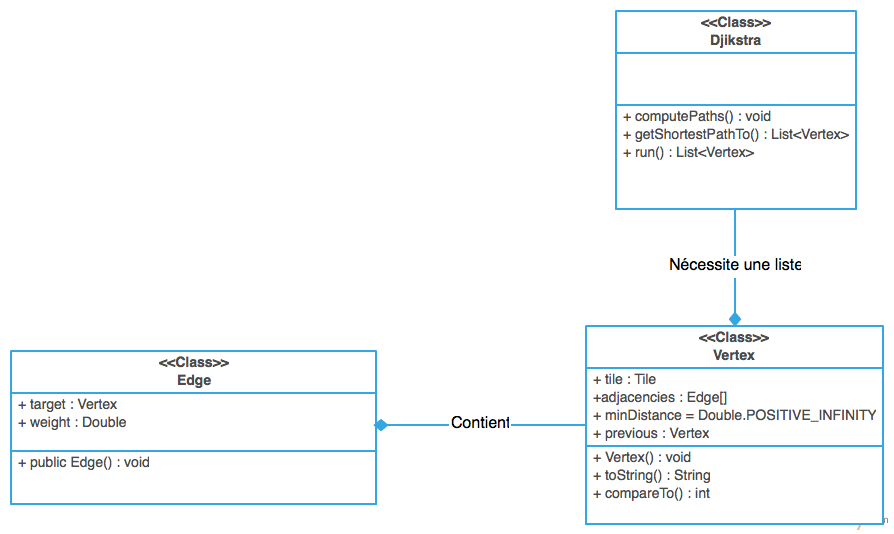
\includegraphics[scale=0.5]{Djikstra}}

Le calcul du plus court chemin se deroule en suivant les étapes qui suivent:
\begin{itemize}
	\item Créer une liste repertoriant tous les noeuds de la carte, c'est-à-dire créer une liste de Vertex;
	\item Pour chaque, noeuds déterminer qui sont ses voisins et le poids du passage du noeud A au noeud B (pas defaut 1). Cela correspond a un tableau de Edge;
	\item Lancer l'algorithme de Dijkstra avec la methode run() en précisant le point de depart et le point point d'arrivé dans les paramètres. 
	\item Le chemin retourné est une liste de Vertex correspondant au chemin à suivre.
\end{itemize}